
\clearpage

\section{Una revisión al ADN}
\label{sec:ADN}


\subsection{Historia del ADN}
La epopeya del ADN tiene sus inicios en 1869 con un bioquímico llamado Friedrich Miescher, esté estaba interesado en la estructura química de las fascinantes unidades fundamentales de la vida conocidas como células.
Miescher viajaba todos los días a la clínica más cercana para tomar las vendas sucias, esto debido a que estaban recubiertas de pus (lo cual era una buena fuente de leucocitos), añadiendo álcali hizo que los núcleos se abrieran liberando sus componentes, de esta manera Miescher extrajo un componente(ADN), al que el nombro nucleína, realizando un análisis de esta nucleína mostró que era un ácido que contenía fósforo y por tanto no calificaba en en ninguno de los grupos conocidos en ese momento como carbohidratos y proteínas, este fue clasificado como un ácido nucleico y su relevancia biológica no fue descubierta hasta mucho tiempo después \cite{Susan}.\\

En 1928 Fredrick Griffith realizaba una investigación con neumococos, tenia dos tipos: el primero patógeno  fue cultivado en placas de petri conocido como s(smooth-suave) debido a su apariencia, el segundo inofensivo y conocido como r(rough-áspero), Griffith descubrio que al añadir un extracto de los neumococos tipos S al tipo R, esté ultimo podría heredar las propiedades del tipo S, este -principio de transformación- indicaba que el extracto contenía la molécula de herencia.\\

Oswald Avery junto con MacLeod y McCarty demostrarón que substancia efectiva en el experimento de Griffiths era la molecula de ADN y que a su vez, era el portador de genes en la célula, también es importante mencionar que Alfred Hershey y Martha Chase quienes confirmaron la conclusión en 1952 mediante experimentos con trazadores radioactivos\cite{Thormod}.\\

Es relevante mencionar otros aportes significativos: \\
1.Erwin Chargaff encontro una regularidad peculiar en los radios de las bases de los nucleotidos.\\
2.Sven Furger trabajo en la estructura de los componentes del ADN, encontró que la base plana(plano de la citocina) era perpendicular a la molecula de azucar.\\
3.Rosalind Franklin logro distinguir dos tipos de ADN dependiendo de la hidratación y que ambos tenían estructura helicoidal mediante cristalográfia, véase figura ~\ref{fig:rf}.

\begin{figure}[htbp]
    \centering
    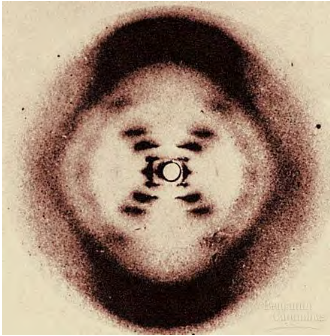
\includegraphics[width=0.5\linewidth]{./Figures/RF.png}
    \caption[Fotografía cristalográfica del ADN]{Fotografiá cristalográfica del ADN tomada por Rosalind Franklin en 1952}
    \label{fig:rf}
\end{figure}
El ultimo paso hacia la estructura del ADN fue llevado acabo por James Watson y Francis Crick en el laboratorio de Cavendish en francia, juntos trabajaron en diferentes modelos de la molécula de ADN , en 1953 publicaron un articulo en la prestigiosa revista Nature titulado: "Molecular Structure of Nucleid Acids", el articulo solo tenia una pagina, pero era de un impacto significativo debido al modelo de ADN que contenía, un modelo de doble hélice(figura ~\ref{fig:jw}), y sugerían que el emparejamiento  especifico que habían postulado intuía un posible mecanismo para copiar material genético.
\begin{figure}[htbp]
    \centering
    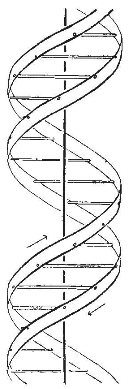
\includegraphics[width=0.15\linewidth]{./Figures/DNA1.png}
    \caption[Diagrama esquemático del ADN]{Diagrama esquemático del ADN publicado por Watson y Crick en 1953, imagen tomada de \cite{jwfc}.}
    \label{fig:jw}
\end{figure}
\subsection{Estructura del ADN}
el ADN es una molécula compuesta por dos largas cadenas, estas cadenas están formadas de múltiples nucleotidos y cada nucleotido esta compuesto por una base una molécula azúcar y un grupo fosfato.\\
El código genético del ADN esta representado por grupos de cuatro tipos de base con secuencias especificas. En el ADN, el azúcar es desoxirribosa, y esta unida a un grupo fosfato,  la base puede ser adenina (A), citosina (C), guanina (G), o timina (T), los nucleotidos están unidos covalentemente en una cadena mediante azúcar y fosfatos, y forman una estructura en forma de cadena alternando azúcar-fosfato-azúcar-fosfato. La estructura tridimensional del DNA(Doble hélice) surge de las características químicas y estructurales de las dos cadenas de nucleotidos. Debido a que las dos cadenas se sostienen juntar debido a los enlaces de hidrógenos entre las base (A y T; G y C), todas las bases se encuentran en el lado interna de las hélices mientas que los grupos azúcar fosfato en la parte exterior\cite{rescells}.

\subsubsection{Daño inducido por radiación al ADN}

 Cualquier forma de radiación tiene el potencial de interactuar con estructuras claves como lo son los átomos para generar ionización, una vez suceda esto se inician eventos en cadena que llevan a cambios biológicos, estos efectos biológicos presentes en algún ser vivo debido a la radiación son relacionados a daños en el ADN.\\
 Esto se conoce como  acción directa de la radiación, y es el proceso dominante para radiación con gran cantidad de transferencia lineal de energía (LET) tales como partículas $\alpha$ o neutrones\cite{rescells}.\\

Por otro lado se tiene la acción indirecta de la radiación, la radiación puede interactuar con los átomos de moléculas de una célula(particularmente con agua) para producir radicales libres, los cuales se pueden difundir lo suficientemente lejos para interactuar con objetivos críticos y causar daños, los radicales libres tienen electrones desapareados lo que causa gran reactividad química. La mayoría de la energía  depositada en células es inicialmente absorbida por el componente principal de las células, el agua, esto conlleva a una producción rápida de
oxidantes y reductores de radicales hidroxilo reactivos. Los radicales hidroxilo pueden difundirse lo suficiente para interactuar con el ADN y causar daños. Afortunadamente, algunos sistemas defensivos o respuestas en las células pueden proteger a las células de los daños\cite{rescells}.\\
\\\

Evidencia acumulada en estudios radiológicos \cite{Franklin},\cite{rescells},  sugieren al ADN como el  objetivo sensible a la radiación. Esto se traduce en lesiones o modificaciones a genes y cromosomas, entender estos cambios son fundamentales para investigar y comprender la carcinogénesis, la muerte celular inducida por la radiación, y la transformación celular.\\


\paragraph{Rompimientos simples}
Un rompimiento simple es un rompimiento en un enlace peptidico, es decir azúcar fosfato, este daño es usualmente fácil de reparar, y en experimentos  se ha demostrado que aproximadamente el 90\% de los rompimientos simples son reparados en el curso de una hora a una temperatura de $37^{\circ} C$ \cite{Thormod}

\paragraph{Rompimientos dobles}

Este tipo de daño involucra las dos cadenas  del ADN, Si el enlace peptidico se rompe a cada lado dentro de una distancia de unos cuantos pares base se presentara un rompimiento doble, estos suelen estar relacionados con muerte celular y daño a los cromosomas.\\
Los rompimientos dobles son posibles de reparar, sin embargo, es mucho más difícil de reparar que un rompimiento simple,
la molécula de ADN contiene proteínas que suportan la estructura y previene que las piezas se caigan incluso cuando un rompimiento ocurre en ambas cadenas del ADN, de hecho, existen un numero de mecanismos que organismos complejos(como los humanos) han evolucionado para reparar los rompimientos dobles\cite{Thormod}.

\begin{figure}[htbp]
    \centering
    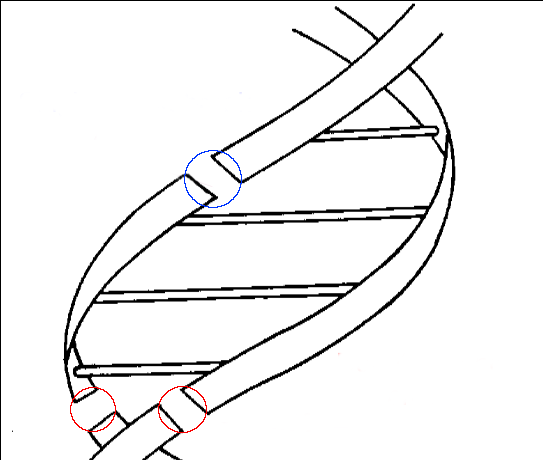
\includegraphics[width=0.5\linewidth]{./Figures/esbdb.png}
    \caption[Esquema rompimientos simples y dobles]{Rompimiento doble en rojo y rompimiento simple en azul, adaptada de \cite{Thormod}}
    \label{fig:esbdb}
\end{figure}


\paragraph{Daño base}

Como resultado de un fallo al reparar o de una falta de reparación, el codon(una secuencia de tres nucleótidos) alterado puede insertar un aminoácido incorrecto en la proteína y a su vez, la proteína modificada podría no funcionar correctamente, Si una base es alterada, la información puede cambiar o perderse,es conveniente mencionar que el daño a la base es uno de los puntos iniciales para la mutación. \\
Experimentos indican que la sensibilidad a la radiación varia de una base a otra. Después de una ionización inicial, rápidas organizaciones electrónicas toman lugar con el resultado de que el daño es transportado a ciertas regiones de la macromolecula (La guanina es particularmente sensible)\cite{Thormod}.

\paragraph{Dimeridos de pirimidina}

Se conoce a dimeridos de pirimidina cuando dos bases adyacentes, (T y T, para la figura ~\ref{fig:dbdi})en la misma cadena se han alterado (sea químicamente o por cualquier otro motivo),  sucede entonces  que se necesita una de las cadenas para replicar la cadena siguiente, como efecto cuando ambas cadenas están dañadas en el mismo sitio no hay manera de que esto se lleve acabo.

\begin{figure}[htbp]
    \centering
    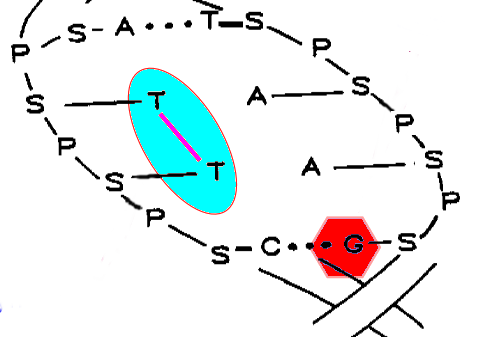
\includegraphics[width=0.5\linewidth]{./Figures/base-piri.png}
    \caption[Esquema Daño base y Dimeridos]{ Daño de la base en rojo y dimeridos de pirimidina en cian, adaptada de \cite{Thormod}}
    \label{fig:dbdi}
\end{figure}

\subsection{Daño Celular}
Antes de seguir es importante aclarar porque es importante el daño ocasionado por radiación ionizante a las células. En general los organismos complejos como los animales y las plantas, están compuestos de células procariotas, estás células contienen la unidad molecular de información conocida como gen el cual se encargada de la herencia genética, o en otras palabras la transferencia de características de los individuos a su descendencia, esta información genética esta codificada por el ADN y es empacada en cromosomas, el conjunto de todos los genes de los cromosomas se conoce como genoma. Lo anterior es relevante debido a que el ADN es extremadamente importante en la replicación celular y un daño a este puede ocasionar aberraciones de cromosomas y mutación de genes, lo que genera subsecuentes efectos biológicos.\\
\\
A su vez también es notable mencionar que la irradiación puede afectar células malignas afectando la estructura, estabilidad, y reparación del ADN, invocando procesos como rompimientos dobles y induciendo efectos terapéuticos contra las células tumorales tales como apoptosis, necrosis,  senescencia, y mitosis anormal como se menciona en \cite{cancer}.\\


%La radiación ionizante se encuentra en nuestro ambiente natural y %también es generada y usada por la humanidad, usos médicos. Un %entendimiento mejor de los efectos biológicos de la radiación %ionizante lleva a un uso y una protección mejor de la radiación. %La respuesta de las células a la radiación sera descrita y %discutida. La significancia de la consecuencias de varios tipos de %radiación inducida-daño de ADN, muestra que el ADN es el principal %blanco para efectos biológicos de la radiación. los daños %reparados mal o que no se reparan, en particularmente en el ADN %los rompimientos dobles, induciran aberraciones de cromosonas y %mutacipon de genes, en la otra mano, la radiación-inducida %rompimientos dobles en el ADN juega un rol importante en la %inducción de apoptosis y punto de control del ciclo celular

\subsubsection{Reparación del ADN}

Los encargados de trabajar en la reparación en las células son las encimas, dependiendo de su función algunas encimas se encargan de ubicar el daño en el ADN mientras que otras son llamadas a reparar el daño, los procesos de reparación pueden ser divididos en tres tipos:\\

1.EL sitio especifico del daño es reparado. En este caso las encimas trabajan directamente en el sitio dañado. La secuencia original de la base se conserva.\\

2. Todo el tramo de ADN que contiene un sitio (o sitios) dañados se eliminan y se reemplazan, preservando la secuencia nativa.\\

3.El daño se ignora durante la replicación; se pasa por alto. Con suerte, se insertará la base correcta o, si es incorrecta, no importará. Debido a que este tipo de reparación es propenso a errores, se mantiene en reserva en caso de que los sistemas de reparación de mayor fidelidad pierdan o no puedan hacer frente al daño. Por esta razón, se llama acertadamente reparación "SOS".\\

\subparagraph{Reparación por escisión}

One important repair mechanism is “excision repair”. This repair mechanism involves enzymes that cut out the damaged part of DNA and replaces it with a new undamaged part.

1. Recognition. It is important to have enzymes that can recognize the damage and signal for help. 2. Cutting of the DNA-strand.
It is a requirement that specific enzymes, like the endonucleases, can cut the DNA-strand in the neighborhood of the damage.
3. The damaged part is removed and rebuilt. Exonuclease and polymerase are key enzymes. The former cuts out the damaged part and polymerase replaces it with a new undamaged part. 4. Joining. The repair is finished when the ligase enzyme joins the cut DNA-strand back together.
The repair system, outlined above, is found in humans and microorganisms.

Genome protection requires the capability to repair DSBs and to ensure that repair is performed with sufficient fidelity. There are two main pathways of DSB repair, namely, homologous recombination (HR) and nonhomologous end joining (NHEJ), which are error-free and error-prone, respectively. The pathways are conserved from Saccharomy cescervisae to mammalian
cells, despite the different relative importance. It is generally considered that HR and NHEJ dominate DSB repairs in yeast and in mammalian cells, respectively. DSB repair has been the subject of a number of excellent reviews [25-31].
\subsubsection{Mecanismos de defensa}

\subsubsection{Respuesta adaptativa}

\subsubsection{Efectos de radiación ionizante en células no irradiadas}
\cite{willmari}
